\section{Detecção de estrelas}
\subsection{Localização de círculos}

Os métodos de detecção de círcurlos em geral consiste nas variações do método de Hough Transform (HT), como o standard Hough Transform, 
o Fast Hough Transform de de Li et al.

Para aplicar um método de Hough Transform, é necessário se aplicar um filtro para detecção de bordas na imagem, 
que filtra apenas os pixels que estão entre na borda das estrelas detectadas, 
pois HT utiliza a posição destes pixels para calcular o possível centro do círculo.
Neste trabalho utiliza-se um filtro clássico de Canny, para realizar a detecção das bordas, 
pois o ganho em qualidade de detecção de outros algoritmos de detecção de borda, como o método de onda contínua, 
que utilizam recursos computacionais maiores, e não aumenta de forma satisfatória a qualidade de detecção de bordas, 
como é mostrado por Kobylin ~\cite[]{kobylin2014comparison}

HT faz utilização da equação do círculo, para fazer a detecção do círculo, o método consiste em se testar todas as possilidades de círculos possíveis para cada pixel na borda de cada ponto na imagem.
Uma vez feito todos os câlculos para cada um dos pixels de borda, o mêtodo seleciona o circulo com maior recorrência em diferentes pixels. Yuen demonstra sua aplicação em diferentes variações ~\cite[]{YUEN199071}.

\subsection{Transformação de coordenadas}

A localização das estrelas ocorre em coordenadas cartesianas em relação ao centro do campo de visão da câmera, 
utilizando o referêncial já demonstrado, porém é mais conveniente que a localização seja representada através de coordenadas polares, 
para isso é necessário se realizar a transformação de coordenadas.
Seguindo as formulas  ~\ref{eq:transformacao_cordenadas_theta} e ~\ref{eq:transformacao_cordenadas_r}.

\begin{equation}
	\theta  = 
	\begin{cases}
		\arctan \left( \frac{y}{x} \right), & \text{se } x >= 0 \\
		\arctan \left( \frac{y}{x} \right) + \pi, & \text{se } x < 0, \\
	\end{cases}
	\label{eq:transformacao_cordenadas_theta}
\end{equation}

\begin{equation}
	r = \sqrt{x^2 + y^2}.
	\label{eq:transformacao_cordenadas_r}
\end{equation}

A variável \textbf{r} é então transformada em uma variável ângular, através de uma relação linear. 
Com os coeficientes sendo calculados através de uma imagem de referência, 
basicamente se faz uma contagem de quantos pixels que se precisa para se percorrer 1 grau de ângulo, para se realizar a medição deste coeficiente,
na Equação ~\ref{eq:transformacao_cordenadas_theta_angular}, r é quantidade de pixels medida na imagem, e C é o coeficiente de transformação, 
\begin{equation}
	r_{angular} = r * C_{converção}.
	\label{eq:transformacao_cordenadas_theta_angular}
\end{equation}

\subsection{Cálculo do ângulos entre estrelas}

O calculo da distância entre as estrelas presentes no FOV é realizado através da Equação ~\ref{eq:calculo_distancia_estrelas}.
Além disto, é aplicado um valor máximo para limitar o ângulo entre as estrelas, pois isto diminui a quantidade de relações armazenadas no banco de dados.
Na Figura ~\ref{fig:angulo_entre_estrelas} é demonstrado as relações entre as estrelas.

\begin{figure}[H]
	\centering
	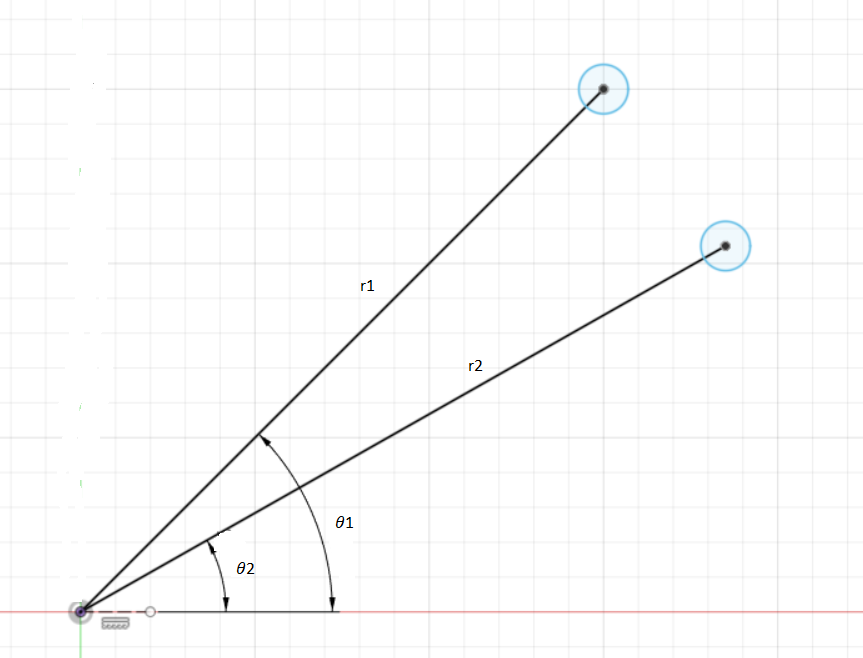
\includegraphics[width=0.5\textwidth]{images/relacoes_entre_estrelas.png}
	\caption{Relação entre estrelas no FOV da câmera, Fonte: Autoria própria}
	\label{fig:angulo_entre_estrelas}
\end{figure}

\begin{equation}
	dist_{angular} = \sqrt{r_{estrela_1}^2 + r_{estrela_2}^2 - 2 * r_{estrela_1} * r_{estrela_2} * cos(\theta_{estrela_1} - \theta_{estrela_2})}
	\label{eq:calculo_distancia_estrelas}
\end{equation}

\subsection{Cálculo da área antre estrelas}

Além da relação angular entre duas estrelas, pode-se calcular a área entre 3 estrelas, 
isto sé faz necessario pois existe uma quantidade grande de estrelas que possuem uma mesma quantidade de estrelas vizinhas a uma mesma distância angular.
Portanto utilizamos uma terceira estrela para se calcular a área entre as estrelas, que é utilizada para refinar as possíveis estrelas no campo de visão.
Para esta calculo é utilizado a fórmula de Heron ~\ref{eq:calculo_area_estrelas}, que pode ser calculada através da distância angular entre as estrelas.
Que já foi calculada na Equação ~\ref{eq:calculo_distancia_estrelas}, previamente executada pelo algoritmo.

\begin{equation}
	area = \sqrt{p(p-a)(p-b)(p-c)},
	\label{eq:calculo_area_estrelas}
\end{equation},
em que \textbf{p} é a metade do perímetro do triângulo, e \textbf{a}, \textbf{b} e \textbf{c} são as distâncias entre as estrelas.

\begin{equation}
	p = \frac{a+b+c}{2}
	\label{eq:calculo_area_estrelas_p}
\end{equation}

Esta divisão do passos para se calcular a área entre as estrelas, 
é realizada pois o calculo do momento entre a estrelas também utiliza o valor \textbf{p}.

\subsection{Cálculo do momento entre estrelas}

Uma filtragem de terceiro grau é realizada para se diminuir ainda mais a quantidade de possíveis estrelas, 
para isso utiliza-se o momento entre as estrelas, que é calculado através da Equação ~\ref{eq:calculo_momento_estrelas},

\begin{equation}
	momento = \frac{area (a^2 + b^2 + c^2)}{36}.
	\label{eq:calculo_momento_estrelas}
\end{equation}

Pode-se utilizar o momento como uma elemento extra de filtragem pois triângulos com areas semelhantes, podem possuir momentos completamente diferentes, como demonstrado na Figura ~\ref{fig:comparacao_entre_triangulos}.

\begin{figure}[H]
	\centering
	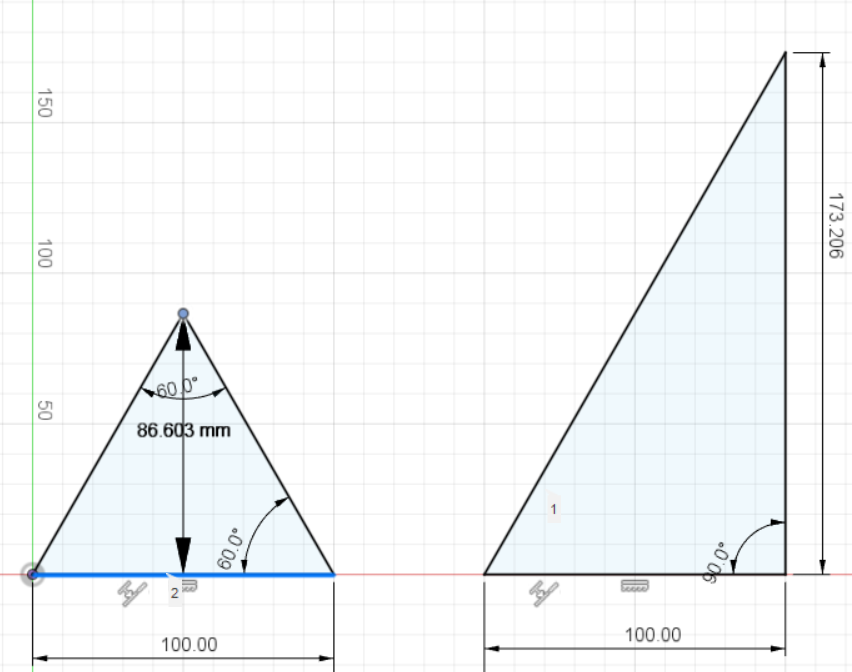
\includegraphics[width=0.5\textwidth]{images/comparacao_entre_triangulos.png}
	\caption{Relação entre estrelas no FOV da câmera, Fonte: Autoria própria}
	\label{fig:comparacao_entre_triangulos}
\end{figure}
Nota-se que esta filtragem é de custo computacional baixo, e utiliza apenas estrelas já analisadas anteriormente, 
portanto é uma passo extra eficaz e de baixo custo computacional.
